\chapter{Metodología}\label{cap:3}
\lettrine{P}{ara modelar el proceso de amplificación} de la semilla de armónicos de alto orden introducida a través del canal de plasma, es necesario plantear y resolver numéricamente las denominadas en la literatura como \emph{\acrlong{mbe}} (\acrshort{mbe}). El código Dagon empleado durante las simulaciones implementa estas ecuaciones mediante un programa escrito en Fortran que, a su vez, está acoplado con otros códigos numéricos ---cuya función se explicará más detalladamente en la sección \S\ref{sec:3.2}---, recibiendo información de partida para iniciar el procedimiento de cálculo. De esta forma, los resultados proporcionan los datos necesarios para comprender cómo afectan la densidad de iones y electrones libres en el plasma a la intensidad y perfil de fase del haz \acrshort{xuv} obtenido. 

Una vez finalizadas las simulaciones, para poder realizar el análisis de las imágenes y los resultados obtenidos, se emplearon dos nuevos programas ---esta vez escritos en Python y Octave---, que permiten almacenar los datos obtenidos en las simulaciones de Dagon y representarlos gráficamente mediante curvas bidimensionales. Además, estos conjuntos de datos pueden introducirse en programas como VisIt para la construcción de imágenes tridimensionales y bidimensionales, por ejemplo, de la propagación del \acrshort{hoh} en la dirección longitudinal del canal.

\section{Ecuaciones de Maxwell-Bloch}\label{sec:3.1}
En este trabajo, el fenómeno físico de la amplificación del armónico inyectado en el plasma de iones de kriptón conduce inevitablemente hasta estas ecuaciones, puesto que determinan cuáles serán las propiedades de la emisión obtenida. Las \acrshort{mbe} describen la dinámica de la interacción entre los modos de vibración de un campo electromagnético y los átomos de un sistema cuántico con dos estados $\left|i\right\rangle$ y $\left|j\right\rangle$. 

El formalismo físico-matemático utilizado en mecánica cuántica para obtener las ecuaciones no es trivial\autocite{cohen-tannoudjiQuantumMechanicsVolume2019,cohen-tannoudjiQuantumMechanicsVolume2019a,Sakurai2020,milonniLasers1988}, aunque tiene la ventaja de predecir con suficiente exactitud la evolución temporal del pulso, además de propiedades físicas de los fotones como su momento angular orbital (\acrshort{oam}), mientras que otros métodos más sencillos ---como el programa de trazado de rayos SHADOX--- no ofrecen esta posibilidad, si bien podría utilizarse para resolver el problema de la amplificación en el plasma. 

En la interacción láser-plasma estudiada, para obtener una buena aproximación basta considerar el campo eléctrico $\symbfcal{E}$ de la semilla \acrshort{hoh}, aunque cálculos más precisos tendrían que incorporar el acoplamiento del campo magnético $\symbfcal{B}$. Además, el acoplamiento entre el campo electromagnético y la materia utiliza una aproximación semiclásica, donde los átomos o iones son sistemas cuánticos de dos estados descritos por la ecuación de Schrödinger, mientras que la luz es un sistema clásico ---una onda electromagnética--- descrito por las ecuaciones de Maxwell.

En primer lugar, el acoplamiento del campo eléctrico con el plasma es la ecuación de ondas 
\begin{equation}\label{eq:3.1}
  \laplacian \symbfcal{E} - \frac{1}{c^{2}}\pdvN{\symbfcal{E}}{t}{2} = \frac{\omega^{2}_{pe}}{c^{2}}\symbfcal{E} + \frac{1}{\epsilon_{0}c^{2}}\pdvN{\symbfcal{P}}{t}{2},
\end{equation}
\noindent
donde el campo eléctrico $\symbfcal{E}$, la polarización $\symbfcal{P}$ y la frecuencia de las oscilaciones del plasma $\omega_{pe}$ son función del espacio y del tiempo, como se dedujo en la sección \S\ref{sec:1.2.2}. 

Como primera hipótesis, se considera la llamada en óptica\autocite{hechtOpticsGlobalEdition2016} como \emph{aproximación paraxial} del campo eléctrico según la dirección de propagación escogida, en este caso, el eje $z$. Suponiendo que la radiación está polarizada linealmente en la dirección del eje $x$, esta simplificación permite tener en cuenta únicamente la componente $x$ del campo eléctrico y de la polarización, dirección en la que oscilarían ambos campos, escribiendo por separado la envolvente y las vibraciones del mismo como
\begin{align}\label{eq:3.2}
  \symcal{E}_{x}(\symbf{r},t) &= \RE \left[E_{+}(\symbf{r},t)\eu^{\iu (kz - \omega t)} + E_{-}(\symbf{r},t)\eu^{\iu (kz + \omega t)}\right], \\
  \symcal{P}_{x}(\symbf{r},t) &= \RE \left[P_{+}(\symbf{r},t)\eu^{\iu (kz - \omega t)} + P_{-}(\symbf{r},t)\eu^{\iu (kz + \omega t)}\right], 
\end{align}
\noindent
donde $E_{+}$, $E_{-}$, $P_{+}$, $P_{-}$ son la amplitud de las oscilaciones de las ondas viajeras hacia la dirección positiva y negativa del eje $z$, respectivamente, es decir, las envolventes. 

Combinando las ecuaciones \eqref{eq:3.1} y \eqref{eq:3.2} y agrupando las componentes que se propagan a lo largo de todo el eje $z$, se obtiene para el campo eléctrico
\begin{align}
  \laplacian \symcal{E}_{x} 
  &= 
  \RE \left[\left(\pdvN{E_{\pm }}{x}{2} + \pdvN{E_{\pm }}{y}{2} + \pdvN{E_{\pm }}{z}{2} + 2k \iu \pdv{E_{\pm }}{z} - k^{2}E_{\pm }\right)\eu^{\iu (kz \mp \omega t)}\right], \\
  \pdvN{\symcal{E}_{x}}{t}{2}
  &= 
  \RE \left[\left(\pdvN{E_{\pm }}{t}{2} \mp 2 \omega \iu \pdv{E_{\pm }}{t} - \omega^{2}E_{\pm }\right)\eu^{\iu (kz \mp \omega t)}\right],
\end{align}
\noindent
obteniéndose el lado izquierdo ($\mathrm{LHS}$) de la ecuación de ondas para el campo eléctrico
\begin{equation}\label{eq:3.3}
  \begin{split}
    \mathrm{LHS} = \RE \Bigg[\Bigg(\laplacian_{\perp}E_{\pm} &+ \pdvN{E_{\pm }}{z}{2} + 2k \iu \pdv{E_{\pm }}{z} - \frac{1}{c^{2}}\left(\pdvN{E_{\pm }}{t}{2} \pm 2 \omega \iu \pdv{E_{\pm }}{z}\right) \\ &+  \left(\frac{\omega^{2}}{c^{2}} - k^{2}\right)E_{\pm }\Bigg)\eu^{\iu(kz \mp \omega t)}\Bigg],
  \end{split}
\end{equation}
\noindent
donde $\laplacian_{\perp}$ es el operador laplaciano transversal actuando sobre el plano $x-y$, es decir, se trata sencillamente de una notación más compacta para escribir 
\begin{equation*}
    \laplacian_{\perp} \equiv \pdvN{E_{\pm }}{x}{2} + \pdvN{E_{\pm }}{y}{2}.
\end{equation*}
La ecuación \eqref{eq:3.3} puede reducirse más simplificando la relación de dispersión del campo eléctrico en el plasma $\omega^{2} = \omega^{2}_{pe} + k^{2}c^{2}\approx k^{2}c^{2}$, puesto que para la emisión de radiación \acrshort{xuv} o rayos X blandos ($\lambda<\qty{40}{nm}$) y la densidad electrónica del plasma de kriptón ($n_e<\qty{e21}{cm^{-3}}$) se tiene que, por un lado, $\omega_{pe}<\qty{1,8e15}{rad/s}$ y, por otra parte, $\omega>\qty{4,7e16}{rad/s}$, luego necesariamente $\omega>\omega_{pe}$ y la aproximación de la relación de dispersión estaría justificada, ya que ambos términos difieren como mínimo en dos órdenes de magnitud. 

Continuando nuevamente con las hipótesis, es importante considerar la aproximación de la envolvente lentamente variable o \emph{\acrlong{svea}} (\acrshort{svea}) que asume la variación temporal y espacial de la envolvente del campo eléctrico lenta\autocite{Larroche2000} comparada con su longitud de onda, de manera que
\begin{align}
  \left|\pdvN{E_{\pm }}{z}{2}\right| &\ll \left|k \pdv{E_{\pm }}{z}\right| \ll \left|k^{2}E_{\pm }\right|,\\
  \left|\pdvN{E_{\pm }}{t}{2}\right| &\ll \left|\omega \pdv{E_{\pm }}{t}\right| \ll \left|\omega^{2}E_{\pm }\right|.
\end{align}

Para ilustrar la importancia del concepto de la \acrshort{svea} en la resolución mediante cualquier algoritmo numérico implementado en un ordenador, la Figura \ref{fig:3.1} muestra esquemáticamente un pulso cuya envolvente ---del campo eléctrico--- varía lentamente, propagándose en la dirección $z$.
\begin{figure}[ht!]
  \centering
  \begin{subcaptionblock}{.4\textwidth}
    \centering
    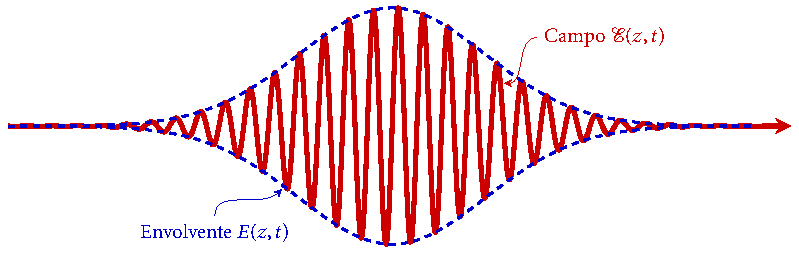
\includegraphics[width=1.2\textwidth]{Figuras/ch3_pulso2d.pdf}
    \caption{Pulso 2D}\label{fig:3.1a}
  \end{subcaptionblock}%
  \begin{subcaptionblock}{.4\textwidth}
    \centering
    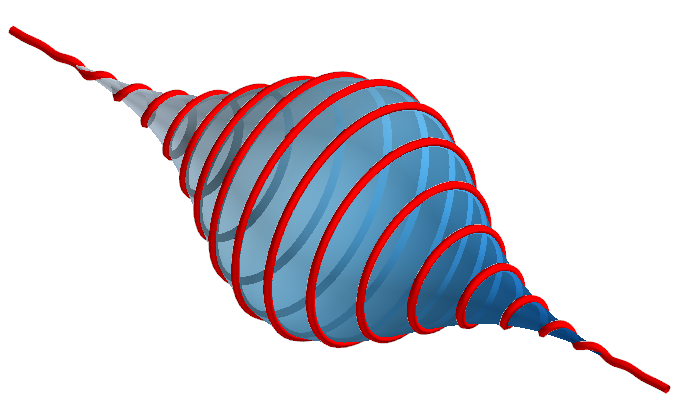
\includegraphics[width=0.8\textwidth]{Figuras/ch3_pulso3d.png}
    \caption{Pulso 3D}\label{fig:3.1b}
  \end{subcaptionblock}%
  \caption{Representación 2D y 3D de un pulso láser con la aproximación \acrshort{svea}.}
  \label{fig:3.1}
\end{figure}

A modo divulgativo, la Figura \ref{fig:3.1b} del pulso 3D ha sido elaborada mediante la escritura del Código \ref{cod:3.1} que recurre a la librería Mayavi de Python para su representación.
\begin{listing}[htbp!]
  \caption{Código escrito para representar una \acrshort{svea} de un pulso 3D.}
  \inputminted[firstline=8, lastline=39]{python}{Programas/mlaser.py}
  \label{cod:3.1}
\end{listing}

Introduciendo estas nuevas hipótesis, la ecuación \eqref{eq:3.3} queda
\begin{equation}
  \mathrm{LHS} =
  \left[\laplacian_{\perp}E_{\pm } - \frac{2 \omega \iu }{c^{2}} \left(\pdv{E_{\pm }}{t} \pm c \pdv{E_{\pm }}{z}\right)\right]\eu^{\iu (\omega t \pm kz)}.
\end{equation}

Para la polarización se realiza su descomposición de forma completamente análoga al campo eléctrico.
\begin{align}
    \pdvN{\symcal{P}_{x}}{t}{2}
    &=
    \left(\pdvN{P_{\pm }}{t}{2} + 2 \omega \iu \pdv{P_{\pm }}{z} + \omega^{2}P_{\pm }\right)\eu^{\iu (\omega t \pm kz)}.
\end{align}

Considerando junto a la SVEA que la amplitud de la polarización en un periodo de la onda es mucho mayor que la variación temporal de su envolvente, es decir,
\begin{equation}
  \left|\pdv{P_{\pm }}{t}\right| \ll |\omega P_{\pm }|,
\end{equation}
\noindent
entonces resulta que
\begin{equation}\label{eq:3.4}
  \pdvN{\symcal{P}_{x}}{t}{2} \approx -\omega^{2}P_{\pm }\eu^{\iu (\omega t \pm kz)}.
\end{equation}

La sustitución de las ecuaciones \eqref{eq:3.3} y \eqref{eq:3.4} en la ecuación \eqref{eq:3.1} permite obtener, tras reordenar los términos a izquierda y derecha
\begin{equation}
  \pdv{E_{\pm }}{t} \pm c \pdv{E_{\pm }}{z} = -\iu \frac{c^{2}}{2 \omega}\laplacian_{\perp}E_{\pm } + \frac{\iu \omega}{2} \left[\left(\frac{\omega_{pe}}{\omega}\right)^{2}E_{\pm } - \mu_{0}c^{2}P_{\pm }\right],
\end{equation}
\noindent
obteniendo una ecuación de advección-difusión-reacción con un término fuente $P_{\pm}$ dependiente del espacio y del tiempo. 

Suponiendo que el tiempo característico de expansión hidrodinámica del plasma es mucho mayor que el de evolución de la polarización, la relación constitutiva procedente de las conocidas en mecánica cuántica como \emph{\acrlong{obe}} (\acrshort{obe}) (términos en la diagonal secundaria de la matriz de densidad para la interacción entre el campo eléctrico y un sistema cuántico de dos niveles) es
\begin{equation}
  \pdv{P_{\pm }}{t} = \Gamma - \gamma P_{\pm } - \frac{\iu z^{2}_{12}}{\hslash }E_{\pm }(N_{2}-N_{1}),
\end{equation}
donde $\Gamma$ es un término fuente estocástico que representa la emisión espontánea, $\gamma P_{\pm}$ es un término sumidero que tiene en cuenta la despolarización del plasma debido a colisiones con electrones libres con $\gamma$ el tiempo característico de variación de la polarización, $z_{12}$ es el término de la diagonal secundaria correspondiente a la matriz dipolar eléctrica y $N_{1,2}$ son las poblaciones de los niveles inferior y superior (los de la diagonal principal de la matriz de densidad). Estos elementos se obtienen a partir de las ecuaciones de tasas
\begin{equation}
  \pdv{N_{1,2}}{t} = \sum_{k} C_{k2,k1}N_{k} \pm \frac{1}{2 \hslash }\IM (E_{\pm }^{*}P_{\pm }),
\end{equation}
\noindent
donde el sumatorio recorre todos los niveles energéticos que participan en las transiciones desde un nivel $k$ hasta los dos estados, incluidas las transiciones entre ambos $k=1, 2$ y $C_{ki}$ son las tasas de excitación y desexcitación del sistema debidas tanto a colisiones como a emisión de radiación. Las poblaciones para los niveles $k\neq 1, 2$ y sus tasas se extraen del código OFK para emplear como entrada de Dagon, como se ha comentado antes.

\section{Esquema computacional}\label{sec:3.2}
Los parámetros de entrada sobre el estado del plasma en el momento de la amplificación necesarios para iniciar Dagon proceden de un código llamado OfiKinRad (OFK). Este código simula la interacción a escala atómica de los constituyentes del plasma, aportando datos sobre la temperatura de los electrones, su densidad, la ionización media, la ganancia y las tasas de colisiones entre iones y electrones.

\section{Esquema experimental}\label{sec:3.3}

\section{Parámetros de las simulaciones}\label{sec:3.4}
